%!TEX root = main.tex

\section{The Method of Steepest Descent}

The method of Steepest Descent is based upon the following property of gradients that we learned in Vector Calculus:

\begin{theorem}
If $f \colon \field{R}^d \to \field{R}$ is continuously differentiable, then at any point $\x \in \field{R}^d$, the vector $-\gradient{f}(\x)$ points in the direction of most rapid decrease for $f$ at $\x$.  The rate of decrease of $f$ at $\x$ in this direction is precisely $-\norm{\gradient{f}(\x)}$.
\end{theorem}

\begin{remark}
For this reason, the vector $\gradient{f}(\x)$ is called the \emph{direction of steepest descent} of $f$ at $\x$.
\end{remark}

In order to search for a local minimum for a twice continuously differentiable function $f\colon \field{R}^d \to \field{R}$, we start by choosing an initial guess $\x_0$.  
\begin{enumerate}
	\item Restrict the function $f$ over the line through $\x_0$ in the direction of $-\gradient{f}(\x_0)$:
	\begin{equation*}
	\varphi_0(t) = f\big( \x_0 - t \gradient{f}(\x_0) \big), \quad t\geq 0
	\end{equation*}
	\item Search for the value of $t_0 \geq 0$ that minimizes $\varphi_0$, and set 
	\begin{equation*}
	\x_1 = \x_0 - t_0\gradient{f}(\x_0)
	\end{equation*}
	\item Repeat this process to get the sequence
	\begin{gather}\label{equation:SteepestDescent}
	\begin{split}
	&\x_{n+1} = \x_n - t_n \gradient{f}(\x_n), \\ &t_n = \argmin_{t\geq 0} \varphi_n(t) = \argmin_{t\geq 0} f\big(\x_n - t\gradient{f}(\x_n)\big)
	\end{split}
	\end{gather}
\end{enumerate}

\begin{remark}
Unlike Newton's method, this algorithm guarantees that $f(\x_{n+1}) \leq f(\x_n)$ for all $n \in \field{N}$.
\end{remark}

\begin{example}
For the polynomial function $p_4(x,y) = x^4-4xy+y^4$ from Example \ref{example:NewtonPoly4}, using the same initial guesses as in Example \ref{example:preNewton4poly4}, we find the following behavior:
\begin{itemize}
	\item Starting at $(x_0, y_0) = (-1.0,1.0)$, the sequence also converges to $(0,0)$, but this time in one step.
	\begin{table}[ht!]
	\begin{tabular}{|r|r|r|r|} \hline 
	$n$ & $x_n$ & $y_n$ & $f(x_n,y_n)$ \\ \hline \hline 
	$0$ & $-1.000000$ & $1.000000$ & $6.000000$ \\ \hline 
	$1$ & $0.000000$ & $0.000000$ & $0.000000$ \\ \hline 
	$2$ & \texttt{nan} & \texttt{nan} & \texttt{nan} \\ \hline 
	\end{tabular}
	\caption{Steepest Descent: Convergence to $(0,0)$ accurately in exactly one step.}
	\label{table:SD00}
	\end{table}
	\item Starting at $(x_0,y_0) = (3.5, 2.1)$, the sequence also converges to $(1,1)$.
	\begin{table}[ht!]
	\begin{tabular}{|r|r|r|r|} \hline 
	$n$ & $x_n$ & $y_n$ & $f(x_n,y_n)$ \\ \hline \hline 
	$0$ & $3.500000$ & $2.100000$ & $140.110600$ \\ \hline 
	$1$ & $1.044472$ & $1.753064$ & $3.310777$ \\ \hline 
	$2$ & $1.141931$ & $1.063276$ & $-1.878163$ \\ \hline 
	$3$ & $1.008581$ & $1.044435$ & $-1.988879$ \\ \hline 
	$4$ & $1.013966$ & $1.006319$ & $-1.998931$ \\ \hline 
	$5$ & $1.000898$ & $1.004472$ & $-1.999891$ \\ \hline 
	$6$ & $1.001437$ & $1.000651$ & $-1.999989$ \\ \hline 
	$7$ & $1.000093$ & $1.000461$ & $-1.999999$ \\ \hline 
	\end{tabular}~\begin{tabular}{|r|r|r|r|} \hline 
	$n$ & $x_n$ & $y_n$ & $f(x_n,y_n)$ \\ \hline \hline 
	$8$ & $1.000149$ & $1.000067$ & $-2.000000$ \\ \hline 
	$9$ & $1.000010$ & $1.000048$ & $-2.000000$ \\ \hline 
	$10$ & $1.000015$ & $1.000007$ & $-2.000000$ \\ \hline 
	$11$ & $1.000001$ & $1.000005$ & $-2.000000$ \\ \hline 
	$12$ & $1.000002$ & $1.000001$ & $-2.000000$ \\ \hline 
	$13$ & $1.000000$ & $1.000001$ & $-2.000000$ \\ \hline 
	$14$ & $1.000000$ & $1.000000$ & $-2.000000$ \\ \hline 
	$15$ & $1.000000$ & $1.000000$ & $-2.000000$ \\ \hline 
	\end{tabular}
	\caption{Steepest Descent: Convergence to $(1,1)$ with 6-digit accuracy in 13 steps.}
	\label{table:SD11}
	\end{table}
	\item Starting at $(x_0, y_0) = (-13.5, -7.3)$, the sequence converges to $(1,1)$, unlike with Newton's Method.
	\begin{table}[ht!]
	\begin{tabular}{|r|r|r|r|} \hline 
	$n$ & $x_n$ & $y_n$ & $f(x_n,y_n)$ \\ \hline \hline 
	$0$ & $-13.500000$ & $-7.300000$ & $35660.686600$ \\ \hline 
	$1$ & $2.362722$ & $-4.871733$ & $640.498302$ \\ \hline 
	$2$ & $1.434154$ & $1.194162$ & $-0.586492$ \\ \hline 
	$3$ & $1.021502$ & $1.130993$ & $-1.896212$ \\ \hline 
	$4$ & $1.038817$ & $1.017881$ & $-1.991558$ \\ \hline 
	$5$ & $1.002305$ & $1.012291$ & $-1.999167$ \\ \hline 
	$6$ & $1.003909$ & $1.001808$ & $-1.999917$ \\ \hline 
	$7$ & $1.000236$ & $1.001246$ & $-1.999992$ \\ \hline 
	\end{tabular}~\begin{tabular}{|r|r|r|r|} \hline 
	$n$ & $x_n$ & $y_n$ & $f(x_n,y_n)$ \\ \hline \hline 
	$8$ & $1.000399$ & $1.000185$ & $-1.999999$ \\ \hline 
	$9$ & $1.000024$ & $1.000127$ & $-2.000000$ \\ \hline 
	$10$ & $1.000041$ & $1.000019$ & $-2.000000$ \\ \hline 
	$11$ & $1.000002$ & $1.000013$ & $-2.000000$ \\ \hline 
	$12$ & $1.000004$ & $1.000002$ & $-2.000000$ \\ \hline 
	$13$ & $1.000000$ & $1.000001$ & $-2.000000$ \\ \hline 
	$14$ & $1.000000$ & $1.000000$ & $-2.000000$ \\ \hline 
	$15$ & $1.000000$ & $1.000000$ & $-2.000000$ \\ \hline 
	\end{tabular}
	\caption{Steepest Descent: Convergence to $(1,1)$ with 6-digit accuracy in 14 steps.}
	\label{table:SD-1-1}
	\end{table}
\end{itemize}
\begin{figure}[ht!]
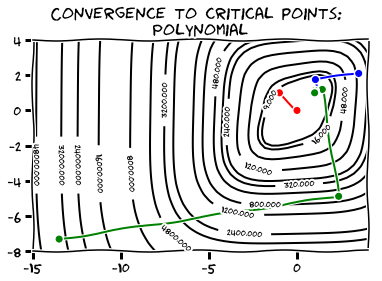
\includegraphics[width=0.6\linewidth]{convergenceSteepest.png}
\caption{The Method of Steepest Descent}
\label{figure:SteepestConvergence}
\end{figure}
\end{example}

\begin{example}\label{example:SDR}
Notice what happens when we try to implement the same process on the Rosenbrock function $\mathcal{R}_{1,1}(x,y) = (1-x)^2 + (y-x^2)^2$, with a wide selection of initial guesses:
\begin{itemize}[nosep]
	\item Starting at $(x_0, y_0)=(-1,-2)$, the method converges to the wrong location: \newline
	\noindent
	\begin{tikzpicture}
	\draw (5.5,0) node{
	\begin{tabular}{|r|r|r|r|} \hline 
	$n$ & $x_n$ & $y_n$ & $f(x_n,y_n)$ \\ \hline \hline 
	$0$ & $-1.000000$ & $-2.000000$ & $13.000000$ \\ \hline 
	$1$ & $0.378555$ & $-1.483042$ & $3.031194$ \\ \hline 
	$2$ & $-0.029793$ & $-0.394111$ & $1.216499$ \\ \hline 
	$3$ & $0.589858$ & $-0.161742$ & $0.427984$ \\ \hline 
	$4$ & $0.589858$ & $-0.161742$ & $0.427984$ \\ \hline 
	$5$ & $0.589858$ & $-0.161742$ & $0.427984$ \\ \hline 
	$6$ & $0.589858$ & $-0.161742$ & $0.427984$ \\ \hline 
	$7$ & $0.589858$ & $-0.161742$ & $0.427984$ \\ \hline 
	\end{tabular}};
	\draw (0,0) node {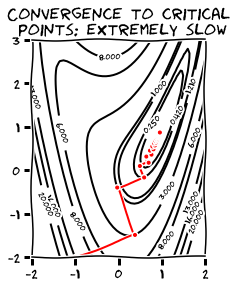
\includegraphics[width=0.35\linewidth]{SDR1.png}};
	\end{tikzpicture}
	\item Starting at $(x_0, y_0) = (0,0.5)$, the method converges very slowly to the actual minimum: \newline
	\noindent
	\begin{tikzpicture}
	\draw (5.2,0) node{
	\begin{tabular}{|r|r|r|r|} \hline 
	$n$ & $x_n$ & $y_n$ & $f(x_n,y_n)$ \\ \hline \hline 
	$0$ & $0.000000$ & $0.500000$ & $1.250000$ \\ \hline 
	$1$ & $0.629348$ & $0.185326$ & $0.181800$ \\ \hline 
	$2$ & $1.000000$ & $0.926629$ & $0.005383$ \\ \hline 
	$3$ & $0.974549$ & $0.939354$ & $0.000756$ \\ \hline 
	$4$ & $1.000000$ & $0.990256$ & $0.000095$ \\ \hline 
	$5$ & $0.996637$ & $0.991937$ & $0.000013$ \\ \hline 
	$6$ & $1.000000$ & $0.998663$ & $0.000002$ \\ \hline 
	$7$ & $0.999539$ & $0.998893$ & $0.000000$ \\ \hline 
	\end{tabular}};
	\draw (0,0) node {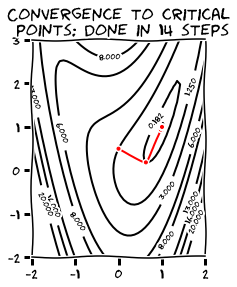
\includegraphics[width=0.35\linewidth]{SDR2.png}};
	\end{tikzpicture}
	\item Starting at $(x_0, y_0)=(-1.9, 2)$, the method gets stuck on the initial guess: \newline
	\noindent
	\begin{tikzpicture}
	\draw (5.4,0) node{
	\begin{tabular}{|r|r|r|r|} \hline 
	$n$ & $x_n$ & $y_n$ & $f(x_n,y_n)$ \\ \hline \hline 
	$0$ & $-1.900000$ & $2.000000$ & $11.002100$ \\ \hline 
	$1$ & $-1.900000$ & $2.000000$ & $11.002100$ \\ \hline 
	$2$ & $-1.900000$ & $2.000000$ & $11.002100$ \\ \hline 
	$3$ & $-1.900000$ & $2.000000$ & $11.002100$ \\ \hline 
	$4$ & $-1.900000$ & $2.000000$ & $11.002100$ \\ \hline 
	$5$ & $-1.900000$ & $2.000000$ & $11.002100$ \\ \hline 
	$6$ & $-1.900000$ & $2.000000$ & $11.002100$ \\ \hline 
	$7$ & $-1.900000$ & $2.000000$ & $11.002100$ \\ \hline 
	\end{tabular}};
	\draw (0,0) node {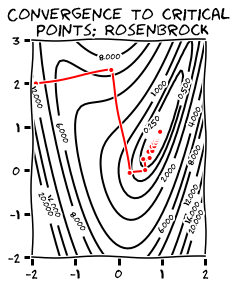
\includegraphics[width=0.35\linewidth]{SDR3.png}};
	\end{tikzpicture}
\end{itemize}
The reason for this behavior lies in the particularly tricky structure of the graph of the Rosenbrock function mainly, but also in the geometry of the Steepest Descent method.
\end{example}

\begin{theorem}
Let $f \colon \field{R}^d \to \field{R}$ be a continuously differentiable real-valued function, and $\{ \x_n \}_{n\in\field{N}}$ a Steepest Descent sequence for $f$.  For any $n \in \field{N}$, $\langle \x_{n+2} - \x_{n+1}, \x_{n+1} - \x_n \rangle = 0$.
\end{theorem}
\begin{proof}
Consider for each $n \in \field{N}$ the function $\varphi_n(t) = f\big(\x_n -t \gradient{f}(\x_x)\big)$, with a global minimum at $t_n \geq 0$.  It must then be
\begin{equation*}
0 = \varphi_n'(t_n) = \langle \gradient{f}(\x_n), -\gradient{f}\big( \x_n - t_n \gradient{f}(\x_n)\big) \rangle = - \langle \gradient{f}(\x_{n+1}), \gradient{f}(\x_n) \rangle,
\end{equation*}
which proves that the gradient of consecutive terms of the Steepest Descent sequence for $f$ are perpendicular.  Now, by virtue of the recurrence formula \eqref{equation:SteepestDescent},
\begin{align*}
\langle \x_{n+2} - \x_{n+1}, &\x_{n+1} - \x_n \rangle = \langle t_{n+1}\gradient{f}(\x_{n+1}), t_n \gradient{f}(\x_n) \rangle \\
&= t_{n+1}t_n \langle \gradient{f}(\x_{n+1}), \gradient{f}(\x_n) \rangle = 0, 
\end{align*}
which proves the statement.
\end{proof}

\begin{remark}
As we saw in Example \ref{example:SDR} with the Rosenbrock function $\mathcal{R}_{1,1}$, the method of Steepest Descent pays a high penalty for moving in perpendicular increments.  
\end{remark}